\section{问题二求解与分析}
\subsection{问题的描述与分析}

场景 B 将同一核心上的全部子图合并为一个 Task。这样，同核子图之间的中间张量可以保留在 L1 或 UB，跨核依赖才需要补入边界 COPY；代价是长期驻留的中间量可能占满私有缓存，迫使核内调度器进一步换入换出。问题一的划分不能直接凭 Task 数少就认定在新场景最优。图~\ref{fig:q2-overview} 对照同核复用、跨核通信以及完整时间线上的选择与验证。

% Generated figure only; description and reference belong before this input.
\begin{figure}[!htbp]
\centering
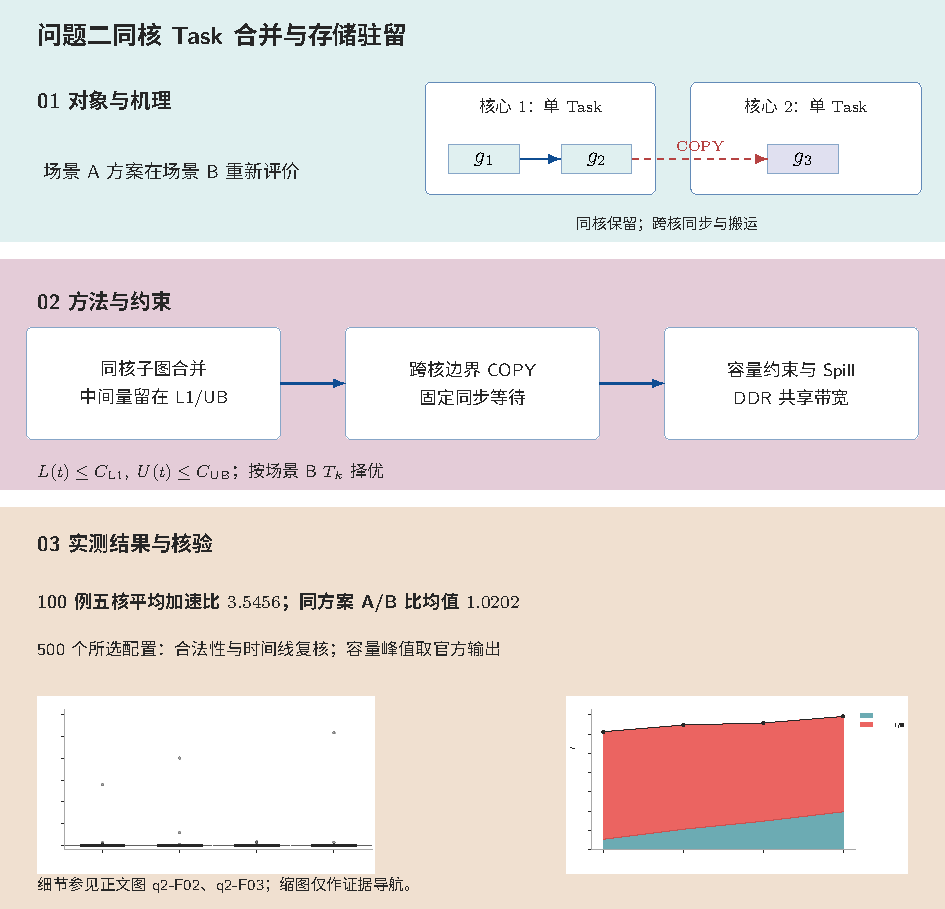
\includegraphics[width=160mm]{../求解/综合图/q2-overview.pdf}
\caption{问题二求解与核验总览}\label{fig:q2-overview}
\end{figure}
\FloatBarrier


图级算子融合可改变中间量的产生、驻留和搬运，TVM的端到端优化框架提供了类似的系统动机\cite{chen2018tvm}。本题场景B的合并对象和缓存语义由官方附件固定；我们仅在合法方案空间中比较它对全局时间线的影响。

\subsection{场景 B 的通信与存储约束}

仍采用问题一的 $g(i)$ 和 $a(g)$。若大小为 $s_j$ 的张量 $j$ 从源操作流向后继操作，且两端归属不同核心，场景 B 须在源核增加 COPY\_OUT、在目的核增加 COPY\_IN；接收端还要等待固定同步延迟。若两端在同一核心，即使所属子图不同，仍可在合并 Task 内保留核内数据，不因子图边界强制插入 DDR 搬运。这个规则与场景 A 的“每过子图边界都搬运”形成核心差别。

对每个时刻 $t$ 和每个核心，记 $L(t)$、$U(t)$ 分别为驻留于 L1 与 UB 的张量字节总量，需满足
\begin{equation}\label{eq:q2-capacity}
L(t)\le C_{\mathrm{L1}},\qquad U(t)\le C_{\mathrm{UB}}.
\end{equation}
其中 L1 容量 $C_{\mathrm{L1}}$ 与 UB 容量 $C_{\mathrm{UB}}$ 都来自题定固定配置。完整 Task 内部的拓扑顺序及必要 Spill 由题定核内调度器确定，所以本式并不等同于只在子图交界检查容量。若合并造成更高的驻留压力，评估器会插入换出与换入；新增 DDR 搬运由原图 COPY、分核边界 COPY 和 Spill 分解核对。

跨核依赖的延迟、共享 DDR 总带宽 $B_{\mathrm{DDR}}$ 及计算 Pipe 占用均按官方多核事件模拟器结算。其输入除了图和配置，只有两个方案字段：操作到子图的映射及各核心子图序列。我们不额外假定跨核 COPY 可以与特定操作完全重叠，也不以缓存可复用等同于缓存必然命中。

\subsection{切图复用与候选比较}

问题二继续采用连通块负载均衡、依赖深度分段以及宽图分批三个候选族，但在场景 B 下分别重评并重新排序。同核分批子图最终合入单个 Task，因此它的额外子图编号不必然造成场景 A 式清空；但分批次序仍可能改变核内拓扑排布和张量存活区间。深度分段虽然切出更多子图，也可能把共享输入关联的操作拉到同核，降低跨核边界；反之，若过多前驱被放到另一核心，则额外 COPY 与同步等待会抵消负载均衡收益。

采用场景B重新择优，对固定核数与算例，按官方场景 B 全局 $T_k$ 选择候选，完成时间并列时比较 $D_k$。为区分硬件规则收益与方案重新选择的收益，另把问题一的选中方案直接放到场景 B 评估，形成同一方案的 A/B 成对时长；场景 B 最优候选相对此固定方案的改善单独报告。两个比较不能混为一个“通信机制增益”。

\subsection{官方算例结果与分析}

场景B的正式结果同样覆盖100例、1至5核及三个预设候选族。图~\ref{fig:q2-f06}按题目要求给出逐例计算后汇总的1至5核平均加速比折线，单核基准与问题一相同。五核平均加速比为3.5456（无量纲），中位数$4.1473$，第10与第90百分位为$1.4066$、$4.9864$。图~\ref{fig:q2-f01}直接给出同一方案从场景A切换到B的逐例时长比，并按核数分层；比值小于1的点表明新场景也可能变慢，不能把均值正向差异解释为每例都获益。场景B五核候选频数为连通块67、深度分段25、分批8；相对场景A有少数算例发生候选切换。

\begin{figure}[htbp]\centering
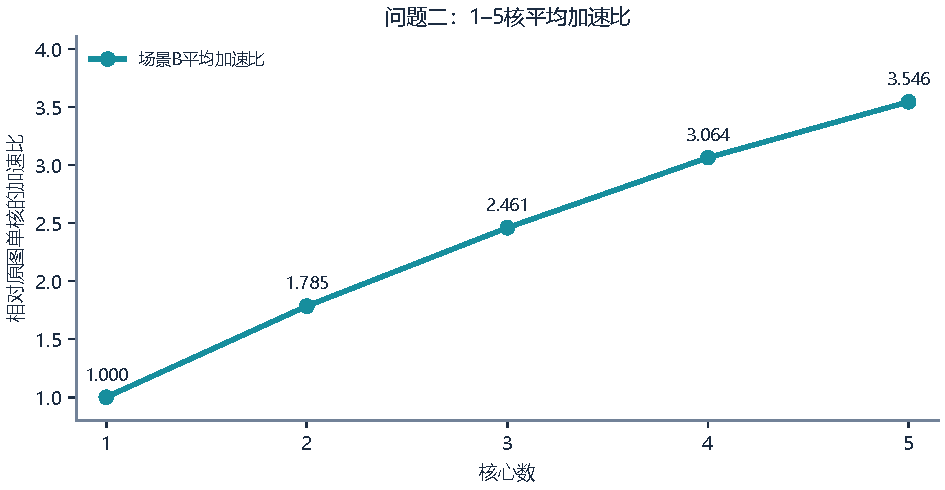
\includegraphics[width=160mm]{../求解/正式图件/q2-F06.pdf}
\caption{问题二核数扩展的平均加速比}\label{fig:q2-f06}
\end{figure}

对应的平均加速比依次为$1.0000,1.7850,2.4605,3.0644,3.5456$。从二核到五核仍持续增长，但相邻核数的绝对增量并不恒定；这些数是100个算例分别求比后的均值，不能把平均完成周期相除来替代。与图~\ref{fig:q1-f02}比较时，两图共用单核基准，因而差别来自场景规则和候选重选的共同作用。后面的同方案对照才将两者拆开。

\begin{figure}[htbp]\centering
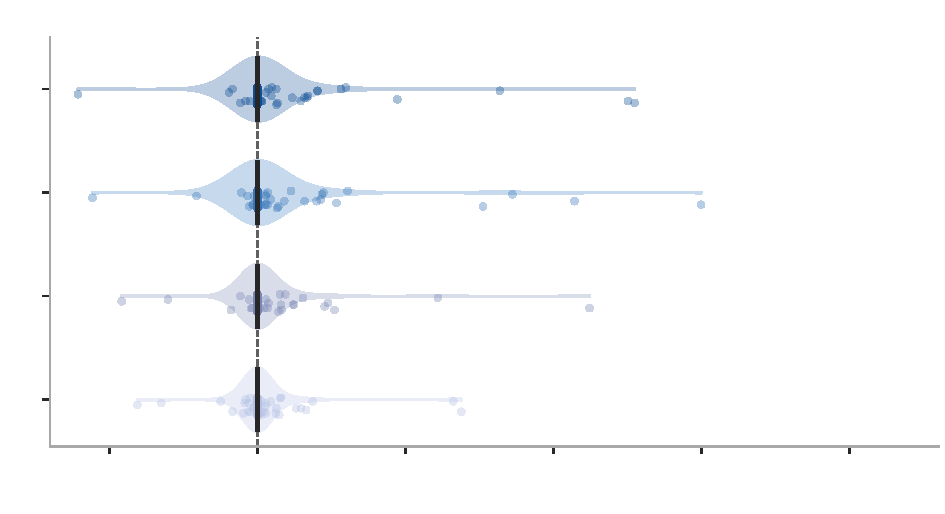
\includegraphics[width=160mm]{../求解/正式图件/q2-F01.pdf}
\caption{同方案场景收益分布}\label{fig:q2-f01}
\end{figure}

为了隔离机制，把问题一选中方案原样放入场景B。五核同方案时长比$T_A/T_B$的均值为$1.0202$，中位数为$1$，最小值$0.7577$，最大值$1.5096$。也就是说，Task合并并不保证逐例加速：个别算例因存储驻留和Spill反而变慢。另以问题二所选候选对同一场景B下的问题一候选作比较，平均再改善$1.0054$倍，中位数仍为$1$。图~\ref{fig:q2-f02}把硬件场景变化和重新择优分开呈现，避免将两种收益叠加成一个笼统结论。

\begin{figure}[htbp]\centering
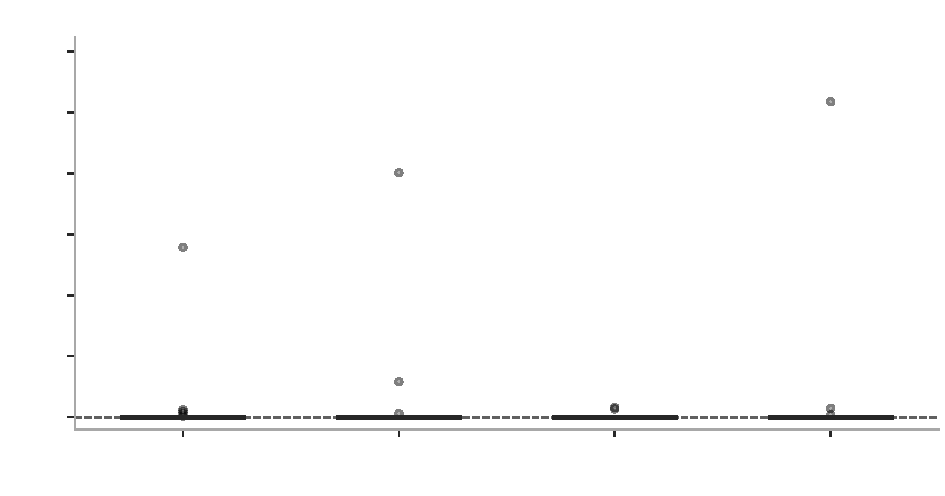
\includegraphics[width=160mm]{../求解/正式图件/q2-F02.pdf}
\caption{场景变化与方案重选}\label{fig:q2-f02}
\end{figure}

图~\ref{fig:q2-f03}按核数分解平均新增DDR搬运，区分切图边界和容量Spill。搬运总量与完成时间并不一一对应：同步等待、共享带宽争用、与计算Pipe的重叠都由事件模拟决定。因此这张图说明成本来源，最终择优仍使用官方全局Makespan。

\begin{figure}[htbp]\centering
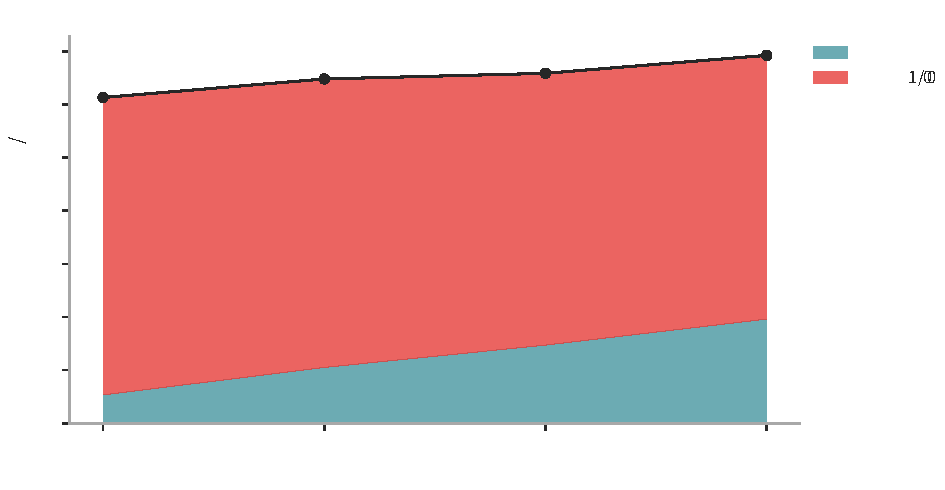
\includegraphics[width=160mm]{../求解/正式图件/q2-F03.pdf}
\caption{新增搬运来源分解}\label{fig:q2-f03}
\end{figure}

问题二的存储约束是逐时刻约束。图~\ref{fig:q2-f04}读取官方详细输出中的五核私有存储最大峰值，除以相应额定容量后同五核加速比对照。该图检视容量压力与调度收益的异质关系；峰值未超过容量只能证明已生成时间线的可行性，不能证明其他未搜索切图也满足约束。图~\ref{fig:q2-f05}则在每个算例的五核成对点上同时表示加速比变化与新增搬运变化；一部分点在“加速且减搬运”象限，但也能看到代价与性能方向不一致的案例，说明不能以搬运字节独立替代完成周期。

\begin{figure}[htbp]\centering
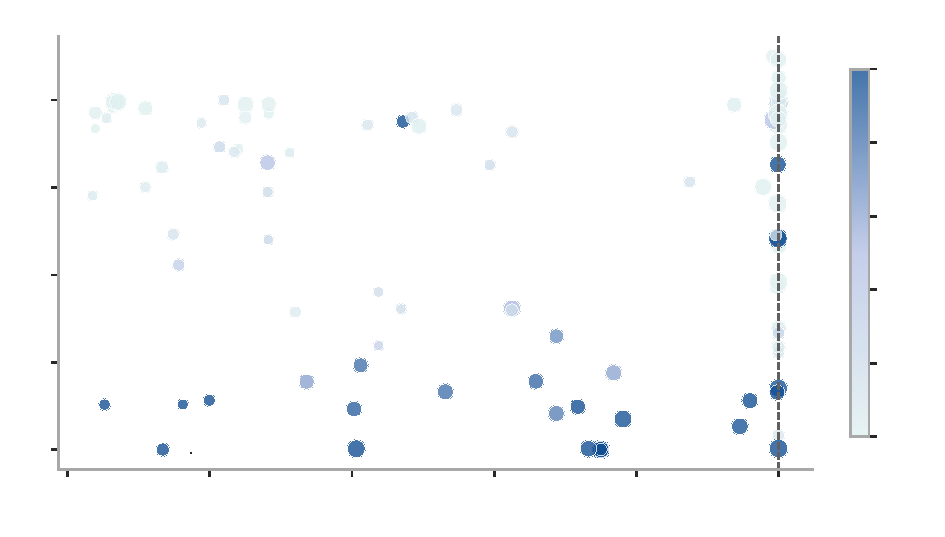
\includegraphics[width=160mm]{../求解/正式图件/q2-F04.pdf}
\caption{容量压力与调度收益}\label{fig:q2-f04}
\end{figure}

\begin{figure}[htbp]\centering
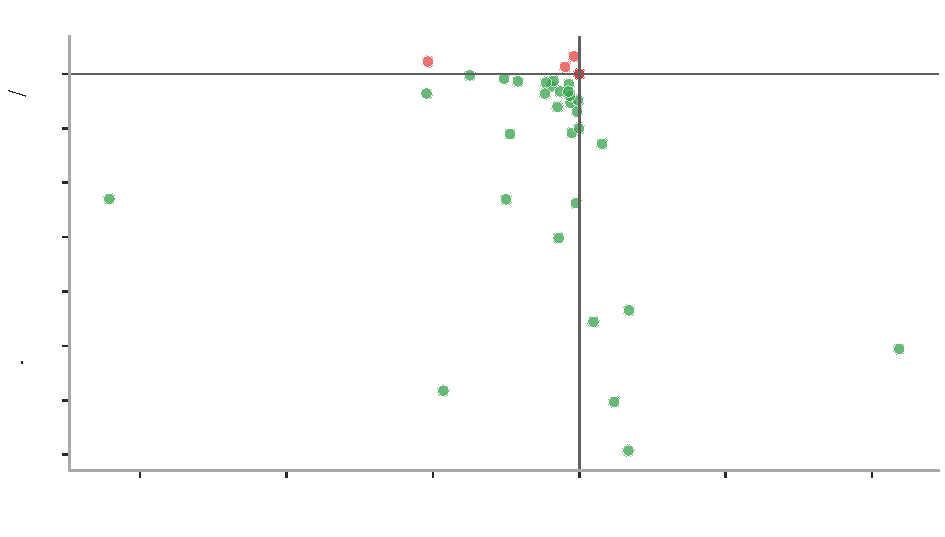
\includegraphics[width=160mm]{../求解/正式图件/q2-F05.pdf}
\caption{加速与搬运的成对变化}\label{fig:q2-f05}
\end{figure}

表~\ref{tab:q2-paired-cases}从两端算例核查两种收益的分离。算例062的两问五核候选都为深度分段，因而$633094/835503=0.7577$直接是同一方案切换场景的比值；场景B虽然比A少了新增DDR搬运，完成周期却增加，说明传输字节下降并不足以保证全局时间缩短。算例071则恰好相反：固定问题一的连通块方案在场景B中仍用$18919$周期，规则本身没有带来时长收益；问题二改选深度分段后才缩至$12470$周期。若只看最后的$1.5172$倍改善，就会把方案适配误写成Task合并本身的效果。

\begin{table}[htbp]\centering
\caption{五核两端算例的同方案与重选对照}\label{tab:q2-paired-cases}
\small
\begin{tabular}{c c r r r r}
\toprule
算例 & 问题一候选 & $T_A$ & $T_B$同方案 & $T_B$重选 & 同方案$T_A/T_B$ \\
\midrule
062 & 深度分段 & 633094 & 835503 & 835503 & 0.7577 \\
071 & 连通块 & 18919 & 18919 & 12470 & 1.0000 \\
\bottomrule
\end{tabular}
\end{table}

上述算例的每个完成周期都来自同一官方事件模拟口径，表中没有用局部Task时间拼接全局Makespan。算例062的逆向差异提示继续检查私有存储驻留、Spill和同步时间；然而现有输出只能证明这些机制共同参与，不能仅凭搬运总量断言某个单项是唯一原因。算例071的重选收益说明场景B下子图划分仍然是决策变量，尽管同核子图最后合入一个Task。

% Generated model comparison; edit scientific report and rerun the builder.
\noindent 本问是有显式约束和官方仿真目标的计算图组合优化；100 个图不提供最优方案标签，直接评价候选方案可复核，学习模型没有可验证的训练目标。\par


\subsection{规则改变与候选重选的逐核分解}

问题二同时更改执行语义与可采用的切图方案，若直接比较问题一、二各自的最优成绩，就无法知道改善来自哪里。对同一算例和核数，记问题一所选方案为$p_A$，问题二所选方案为$p_B$。本文实际保存三次可比评价：场景A的$T_A(p_A)$、场景B但固定方案的$T_B(p_A)$，以及场景B重选后的$T_B(p_B)$。逐例有精确恒等式
\begin{equation}\label{eq:q2-decompose}
\frac{T_A(p_A)}{T_B(p_B)}=
\underbrace{\frac{T_A(p_A)}{T_B(p_A)}}_{\text{规则效应（同方案）}}
\underbrace{\frac{T_B(p_A)}{T_B(p_B)}}_{\text{重选效应（同场景）}}.
\end{equation}
它只是同一实例中三个实测时间的代数分解，并未假设两种效应独立。汇总100例时必须先逐例计算比值再求均值；一般来说，两个逐例因子的均值之积不等于总比值的均值，更不能把三问各自报告的平均加速比直接相除当作式~\eqref{eq:q2-decompose}的第一项。

表~\ref{tab:q2-paired-deep}把二至五核逐级列出。表中“改善/变差”只比较同一方案下的场景A与B，“重选受益”只比较两个场景B方案；等于1的案例不计入任一方向。二核有21例在规则改变后改善、13例变差，五核为24例改善、6例变差，仍有70例无时长变化。五核规则效应的逐例平均为$1.0202$，但其最小值在算例062只有$0.7577$，所以“合并Task平均有益”不能改写成“合并Task对每张图有益”。二至五核的重选受益例数仅5、3、2、3，均值接近1；这是当前三个有限候选族之间的观察，既不说明场景B无需优化，也不表示所有合法划分已被比较。

\begin{table}[htbp]\centering
\caption{场景B逐核成对比较与搬运来源}\label{tab:q2-paired-deep}
\small\begin{tabular}{rrrrrrr}\toprule
核数 & 同方案均值 & 改善/变差例数 & 重选均值 & 重选受益例数 & 候选切换 & Spill例数 \\ \midrule
2 & 1.0053 & 21/13 & 1.0031 & 5 & 7 & 44 \\
3 & 1.0097 & 20/7 & 1.0046 & 3 & 5 & 40 \\
4 & 1.0217 & 23/8 & 1.0003 & 2 & 2 & 37 \\
5 & 1.0202 & 24/6 & 1.0054 & 3 & 3 & 37 \\
\bottomrule\end{tabular}\end{table}


候选族切换次数与重选严格受益次数不同，也值得分开读。二至五核分别有7、5、2、3个案例改变了胜出候选族，超过同核数严格时长改善的5、3、2、3例，说明某些不同族候选在官方全局时长上并列，需靠次级搬运量或固定平局规则确定最终方案。即使候选族不变，具体核心指派也可能变；表中的“切换”只统计族名，不能充当逐字节的方案身份校验。另一方面，五核算例002在固定深度分段方案时由场景A的$83172$周期降到场景B的$55096$周期，比值$1.5096$，而重选因子恰为1。这与前述算例071构成相反的机制示例：002主要见到规则变化的实测收益，071的$1.5172$倍则主要来自场景B重新选出分段方案。两例共同说明必须保留式~\eqref{eq:q2-decompose}的中间评价。

\subsection{边界搬运、Spill与驻留约束}

场景B省去同核子图之间的重复外存往返，但不会让跨核边界和私有存储容量消失。把一个跨核张量的发送端、接收端视为有序依赖，只有两端核心不同才需要跨核边界COPY；这可以用指示量 $I_{uv}=\mathbf 1\{a(g(u))\ne a(g(v))\}$ 标记。张量边的大小与$I_{uv}$乘积有助于候选构造时识别潜在边界流量，但不等于最终的官方新增搬运总量：原始COPY、张量复用次数、Spill以及评估器的具体图转换规则都要计入。本文因此仅以该量作代理，不拿它替换真实 $D_k$，结果图~\ref{fig:q2-f03}用官方详细响应把边界COPY和Spill分开。

核内驻留同样是时间相关约束。若 $\mathcal L_k(t)$ 和 $\mathcal U_k(t)$ 分别表示核心$k$在事件时刻$t$仍位于L1和UB的张量集合，合法峰值要求 $\sum_{j\in\mathcal L_k(t)}s_j\leq C_{\rm L1}$ 与 $\sum_{j\in\mathcal U_k(t)}s_j\leq C_{\rm UB}$ 在全部实际时刻成立。不能把一个Task里出现过的所有张量静态相加当作峰值，也不能用平均占用率取代峰值。合并Task使同核边界数据可能延长驻留时间；即使跨核COPY字节下降，私有缓存更早溢出也可能出现Spill，进而改变DDR请求排队与计算Pipe的空闲区间。本文用官方输出中的逐核峰值与Spill字节核验这一点，没有另造一个与官方事件顺序不一致的内存模拟器。

五核正式所选方案的100例汇总中，新增边界搬运约$392.3$ MiB，Spill约$992.1$ MiB；按这两项总量计算，Spill占新增搬运约$71.7\%$。这是字节量的跨案例求和，不是“71.7\%的案例发生Spill”：五核实际有37例Spill大于零。两个统计口径不同，正说明少数较重的存储压力图可主导总字节数。二至五核发生Spill的例数为44、40、37、37；随核数增加这个计数略降，而边界搬运总量上升，不能据此推出某一种机制单独决定完工时间。图~\ref{fig:q2-f04}的容量峰值与收益散点以及图~\ref{fig:q2-f05}的速度—搬运双轴，分别用于检验上述容量与时间响应是否一致。

\subsection{候选族内的存储代价交叉核查}

总字节均值还有一个隐患：不同类型的图规模和结构混在一起。表~\ref{tab:q2-family-crosscheck}按五核问题二最终胜出的候选族重新分组，分别计算官方详细输出中的边界搬运和Spill平均量，并给出相应案例的平均加速比。这是事后条件描述，不能被解释为把同一批图随机分配到三种算法后的处理效应；尤其某一族只会在它相对有利的图上成为胜者。分组表的意义是核对“哪类已选方案携带怎样的实际资源账”，而不是据均值挑一个永远最优的算法。

\begin{table}[htbp]\centering
\caption{五核胜出候选族的搬运组成与收益}\label{tab:q2-family-crosscheck}
\small\begin{tabular}{lrrrrr}\toprule
候选族 & 例数 & 边界搬运均值/MiB & Spill均值/MiB & Spill例数 & 平均加速比 \\ \midrule
连通块 & 67 & 2.98 & 6.59 & 22 & 3.9476 \\
深度分段 & 25 & 2.69 & 4.15 & 8 & 2.1728 \\
分批 & 8 & 15.68 & 55.85 & 7 & 4.4693 \\
\bottomrule\end{tabular}\end{table}


连通块族在67例中胜出，其边界搬运均值$2.98$ MiB，Spill均值$6.59$ MiB，22例Spill大于零，平均加速比$3.9476$。深度分段族对应25例，边界均值$2.69$ MiB、Spill均值$4.15$ MiB，平均加速比却仅$2.1728$。不能据此称分段“比整块慢”，因为分段主要被难以整块并行的高连通图选中，所面对的图结构不同。分批族只有8例，平均加速比$4.4693$，但边界和Spill均值高达$15.68$与$55.85$ MiB，7例发生Spill。这些案例能凭自身图宽与短任务取得明显并行收益，同时承担很高的绝对搬运成本；高收益与高搬运在不同图规模下完全可以共存。

分组结果还解释了为何只在同一图、同一核数下比较候选，不能把表内三个族的平均加速比直接排序作为部署规则。严格的候选比较需要固定图、硬件参数和核数，然后把每个合法候选交给同一官方评估链。表~\ref{tab:q2-family-crosscheck}没有替代这一步，而是对最终选择作资源诊断。若后续要检验“分段是否降低Spill”这类因果命题，需在同一批案例上保留所有候选的Spill、峰值与时间，并显式处理不合法或超时候选；目前的胜出族条件均值尚不足以给出该结论。

官方详细响应、所选方案和独立核验记录的关联也遵循这个单位：同一案例的二至五核四个方案各自保存，不借用其它核数的时间线。核验程序首先检查非COPY操作覆盖与编号、收缩图无环和同核次序，再比对官方给出的全局完成周期、峰值与新增搬运拆分。出现候选评估失败时，不把缺失时间记为零或无穷大后参与均值；选中方案必须有可读取的官方成功响应。本次500个所选配置全部通过逐项交叉核验，这一通过数反映的是结果可复查性，不是未选候选的全局最优性证明。

\subsection{可迁移结论的范围}

这些逐核比较只针对题目给出的100张图、固定硬件配置和当前候选集合。对同核边界密集且仍有存储余量的图，合并Task可能减少DDR往返；对长寿命张量多、原已逼近L1或UB容量的图，同一改变也可能增大Spill。这个判断是从已观测的成对结果、搬运分解及题定机制提出的条件性解释，不是对任意NPU的性能保证。若移到另一处理器，必须先重测固定等待、私有容量、COPY转换与带宽争用，之后再比较$T_A(p_A)$、$T_B(p_A)$和$T_B(p_B)$；单纯复用本文的胜出频数不能代表新设备的最优策略。当前研究在五核处仍有部分案例由分段候选胜出，表明跨核边界的位置与同核驻留应在后续候选中联合优化，而不是只减少一种COPY数量。

\subsection{容量与时间线核验}

独立核验重新读取官方输出中的操作时间线，确认所选方案的合法性与完成周期一致。张量驻留峰值和COPY分解取自官方详细输出；其中L1、UB峰值均在题定容量内，本文没有对这两个峰值另写独立内存模拟器。独立重算后，所选五百组方案的覆盖、时间线及官方响应交叉核验全部通过。逐例增核并非单调：场景B有24个算例在至少一次增核时加速比下降，与固定同步及内存压力的解释相符，但不能仅凭该计数把原因归结为某一种COPY。

成对比较仍有两项边界：第一，所比的场景均由官方模拟器定义，未测真实硬件上的温度、功耗或抢占；第二，当前候选未针对UB/L1驻留区间显式优化，因此在Spill较重的图上可能还有改善空间。

对式~\eqref{eq:q2-decompose}的逐核结果还应检查“没有变化”的案例。二核固定方案切换场景后，21例严格变快、13例严格变慢，其余66例完成周期相等；五核相应为24例、6例和70例。均值略大于1并不表示大多数图都变快，而是少数受影响案例的幅度足以改变平均值。相等只说明官方全局Makespan未变，不能证明Task边界、COPY数量或私有驻留轨迹也完全相同：这些局部变化可能发生在非关键路径上。因此，评价场景B时同时保留逐例方向、完成周期和搬运拆分，比只报告一个平均倍数更能识别适用范围。

资源账也显示核数增加后的两种压力方向并不一致。按官方详细响应跨100例求和，二核所选方案的新增边界搬运约$106.8$~MiB、Spill约$1119.1$~MiB；五核分别约$392.3$~MiB和$992.1$~MiB。跨核边界总量增加，而Spill总量下降；这不能简化为“增核节省存储”或“增核只增加通信”。两组总量比较使用了不同核数下各自重新选出的方案，且聚合字节无法表示关键路径等待，故只能作为资源诊断。若要在新设备上预先约束最坏延迟或DDR预算，还须以逐图成对评估重新估计尾部风险，不能按本题总体均值直接指定核数。






